\chapter{Metodología de trabajo}

En este capítulo se profundizará en el dominio del problema que se quiere resolver, examinando la metodología a seguir para poder llevar a cabo este proceso, así como las tecnologías y herramientas que se utilizarán para que sea posible su desarrollo.

% ********************************************************************

\section{Complejidad del problema a resolver}

La principal complejidad que presenta el análisis de \textit{logs} es, sin duda, la gran heterogeneidad que tiene su representación, así como la estructura abstracta de algunos de sus campos. En el caso de Linux, esta abstracción viene dada por el campo \textit{message}, probablemente el más importante, ya que este contiene la descripción del evento registrado.

\vspace{-1mm}

\begin{figure}[H]
    \centering
    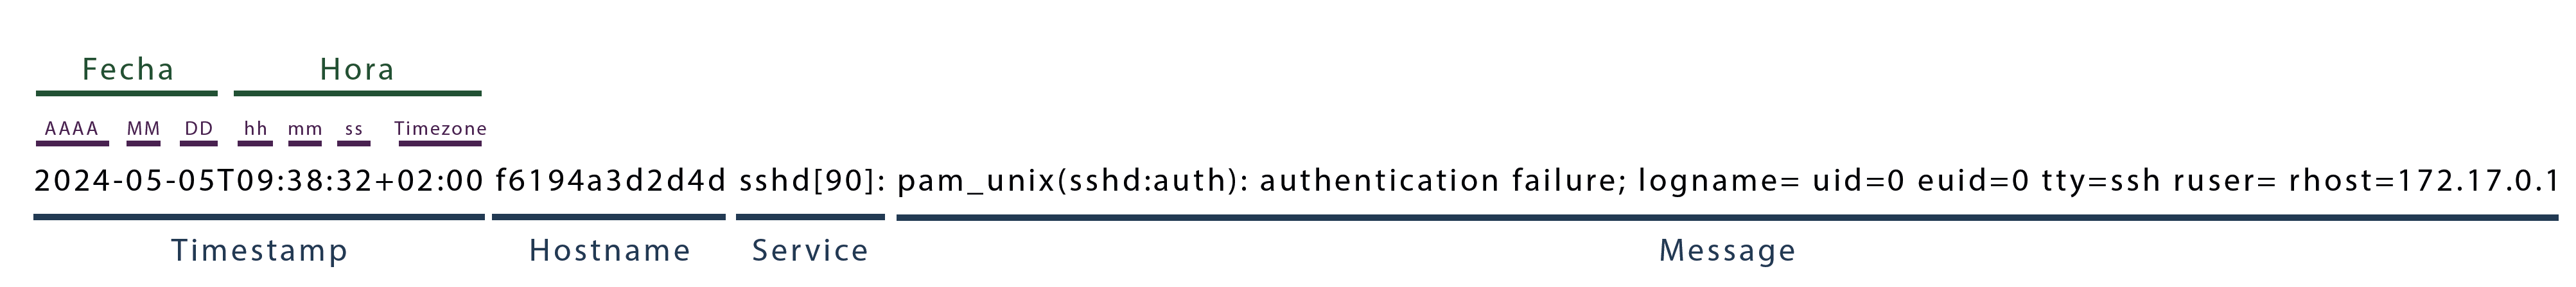
\includegraphics[width=1\linewidth]{imagenes/linux-log-structure.png}
    \caption{Sintaxis de un \textit{log} de Linux}
    \label{fig:linux-log-structure}
\end{figure}

\vspace{-0.5mm}

Como se puede observar en la Figura \ref{fig:linux-log-structure}, los \textit{logs} de Linux presentan un total de 4 campos: \textit{timestamp}, \textit{hostname}, \textit{service} y \textit{message}. Este último representa un claro aumento en la complejidad de preprocesamiento ya que no sigue un patrón concreto sino que esta elección se delega al servicio que está sirviendo la información, como ocurre en la Figura \ref{fig:linux-log-structure-message}.

\vspace{-0.5mm}

\begin{figure}[H]
    \centering
    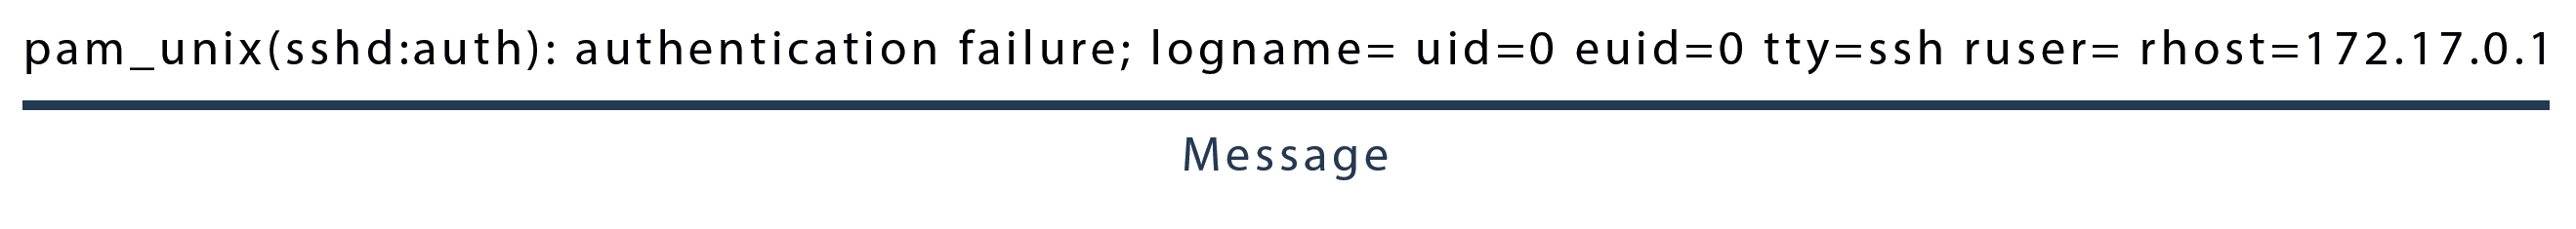
\includegraphics[width=1\linewidth]{imagenes/linux-log-structure-message.png}
    \caption{Sintaxis del \textit{message} de un \textit{log} de Linux}
    \label{fig:linux-log-structure-message}
\end{figure}

Dentro del mismo puede extraerse otra información útil; en el ejemplo proporcionado se informa de un fallo en la autenticación, así como la \gls{tty} utilizada, la \gls{IP} del host remoto involucrado o el identificador de usuario asociado.

Por otro lado, la sintaxis del \textit{timestamp} sigue el formato \gls{ISO} 8601 \cite{iso8601}, el cual consta de la estructura representada en la Figura \ref{fig:linux-log-structure-timestamp}. Analizando los elementos por lo que se compone, se extrae la siguiente información:

\begin{table}[H]
\centering
\footnotesize
\begin{tabularx}{\textwidth}{|>{\raggedright\arraybackslash}p{3cm}|>{\raggedright\arraybackslash}X|}
\hline
\rowcolor{graylight}\texttt{Campo} & \texttt{Descripción} \\
\hline
Fecha & La parte de la fecha está representada en el formato \texttt{YYYY-MM-DD}, donde:
\begin{itemize}
    \item \texttt{YYYY} representa el año en cuatro dígitos.
    \item \texttt{MM} representa el mes en dos dígitos (01 a 12).
    \item \texttt{DD} representa el día del mes en dos dígitos (01 a 31).
\end{itemize} \\
\hline
Hora & La parte de la hora sigue el formato \texttt{hh:mm:ss}, donde:
\begin{itemize}
    \item \texttt{hh} representa la hora en formato de 24 horas (00 a 23).
    \item \texttt{mm} representa los minutos (00 a 59).
    \item \texttt{ss} representa los segundos (00 a 59).
\end{itemize} \\
\hline
Separador & La letra \texttt{T} se utiliza como delimitador entre la fecha y la hora, indicando que la información que sigue es la hora correspondiente a la fecha especificada previamente. \\
\hline
Zona horaria & La parte final del \textit{timestamp} indica la diferencia con respecto al Tiempo Universal Coordinado (\gls{UTC}), expresada en el formato \texttt{±hh:mm}. Por ejemplo, \texttt{+02:00} indica que la hora está dos horas adelantada con respecto a \gls{UTC}. \\
\hline
\end{tabularx}
\caption{Descripción del formato de \textit{timestamp} según el estándar ISO 8601 \cite{iso8601}}
\label{tab:timestamp-format}
\end{table}

\begin{figure}[H]
    \centering
    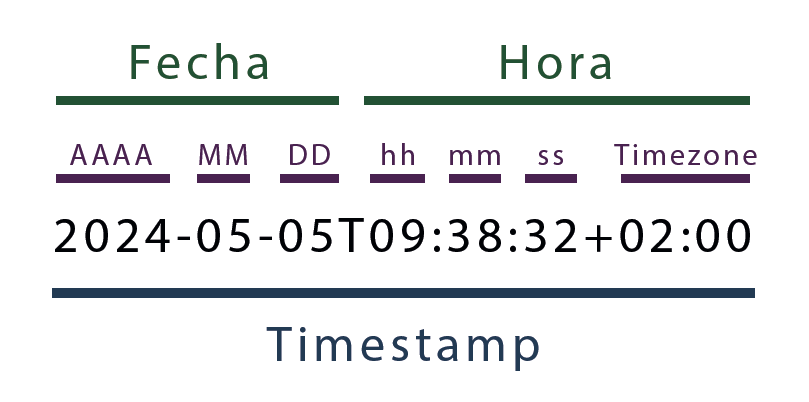
\includegraphics[width=0.6\linewidth]{imagenes/linux-log-structure-timestamp.png}
    \caption{Estructura del \textit{timestamp} de un \textit{log} de Linux}
    \label{fig:linux-log-structure-timestamp}
\end{figure}

Para este proyecto, se hará uso de otros \textit{datasets} de \textit{logs} que contienen una sintaxis que difiere bastante con la ofrecida por \textit{syslog}, por lo que será necesario llevar a cabo un pre-procesamiento de todos los tipos de eventos para que sean homogéneos, de modo que el modelo pueda interpretarlos de forma correcta. \\

En el caso de \gls{BGL}, como se puede observar en la Figura \ref{fig:bgl-log-structure}, existen nueve campos, aunque algunos de ellos redundantes: \textit{timestamp (epoch-time)}, \textit{date}, \textit{service}, \textit{detailed-timestamp}, \textit{hostname}, \textit{compontent}, \textit{severity}, \textit{type} y \textit{message}. De aquí se puede extraer que se repiten los cuatro campos de los \textit{logs} de Linux, y se añaden otros que pueden resultar muy útiles: la severidad y el tipo de evento.

\begin{figure}[H]
    \centering
    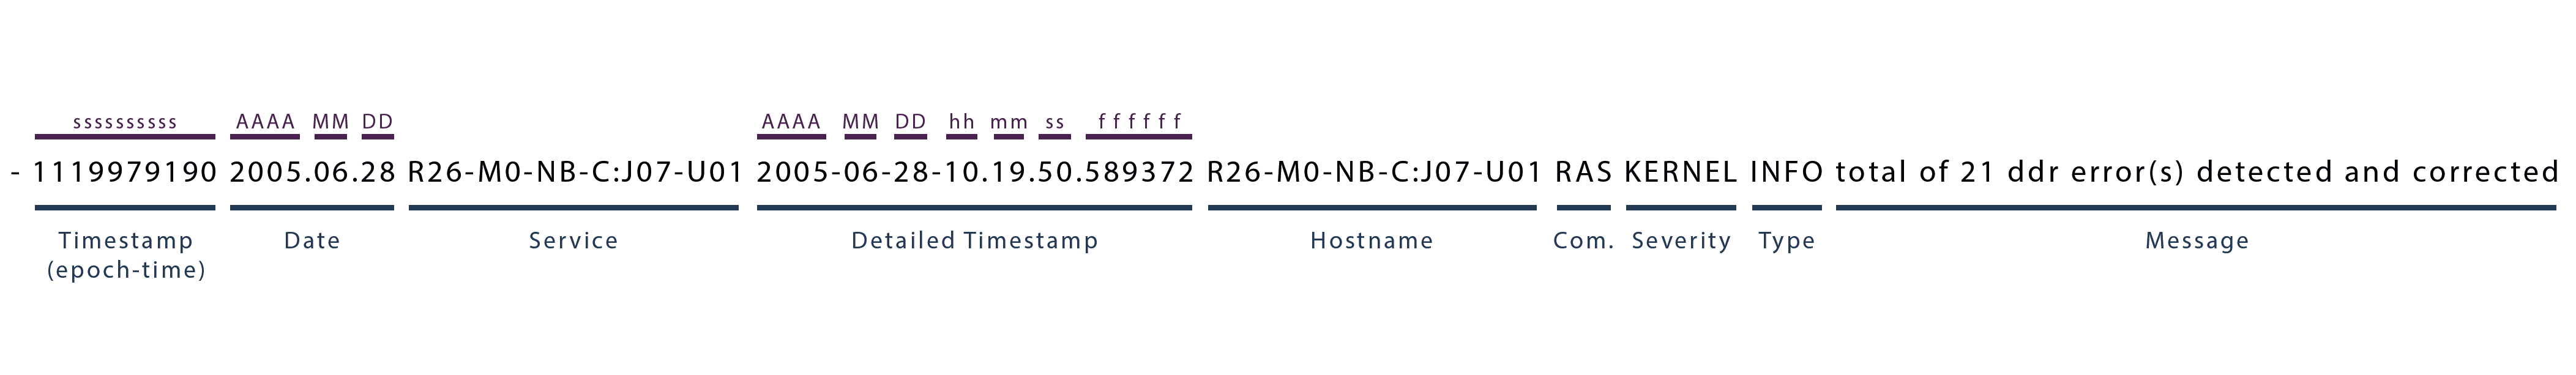
\includegraphics[width=1\linewidth]{imagenes/bgl-log-structure.png}
    \caption{Sintaxis de un \textit{log} de \gls{BGL}}
    \label{fig:bgl-log-structure}
\end{figure}

Otro factor a tener en cuenta es que cambia la estructura del \textit{timestamp}, analizando la Figura \ref{fig:bgl-log-timestamp}, se observa que los delimitadores son guiones y puntos, y que también contiene un campo extra asociado a una mayor precisión en el momento de captura del evento, ya que también mide a nivel de microsegundos, pero se pierde la precisión de la zona horaria.

\vspace{-1mm}

\begin{figure}[H]
    \centering
    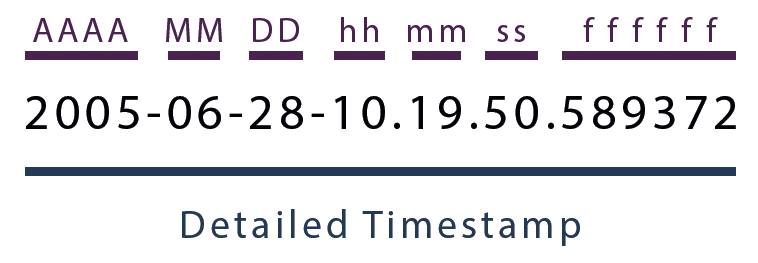
\includegraphics[width=0.6\linewidth]{imagenes/bgl-log-structure-timestamp.png}
    \caption{Estructura del \textit{timestamp} de un \textit{log} de \gls{BGL}}
    \label{fig:bgl-log-timestamp}
\end{figure}

Por último, en el caso de \gls{HDFS}, según se ilustra en la Figura \ref{fig:hdfs-log-structure} los eventos se organizan en cuatro campos: \textit{timestamp}, \textit{thread ID}, \textit{type} y \textit{message}. El único campo nuevo es el identificador de la hebra, aunque no es relevante para el estudio que se está llevando a cabo.

\vspace{-1mm}

\begin{figure}[H]
    \centering
    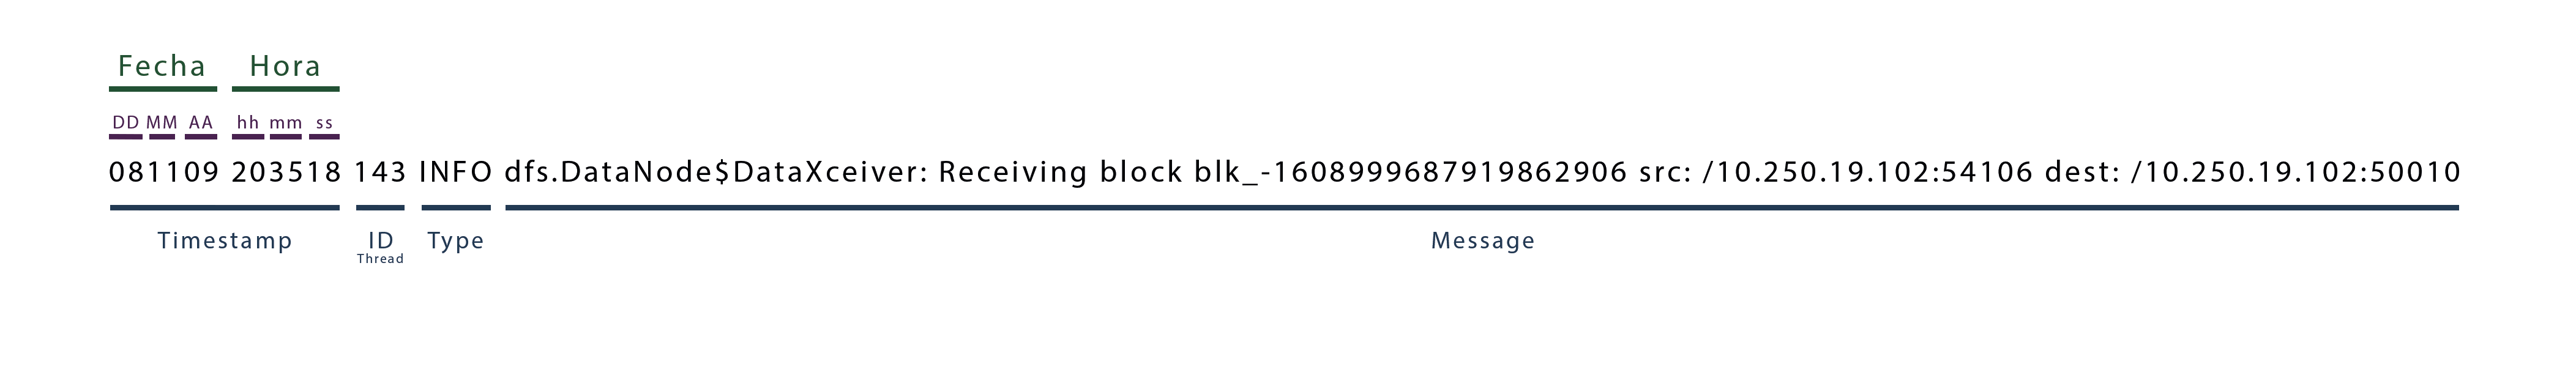
\includegraphics[width=1\linewidth]{imagenes/hdfs-log-structure.png}
    \caption{Sintaxis de un \textit{log} de \gls{HDFS}}
    \label{fig:hdfs-log-structure}
\end{figure}

También varía cómo se organiza el campo de \textit{timestamp}. Según se ve en la Figura \ref{fig:hdfs-log-structure-timestamp}, este es menos preciso en comparación con los anteriores, pero sigue siendo útil para llevar a cabo el estudio. Además, también se mantiene el campo \textit{message} con una estructura irregular.

\vspace{-1mm}

\begin{figure}[H]
    \centering
    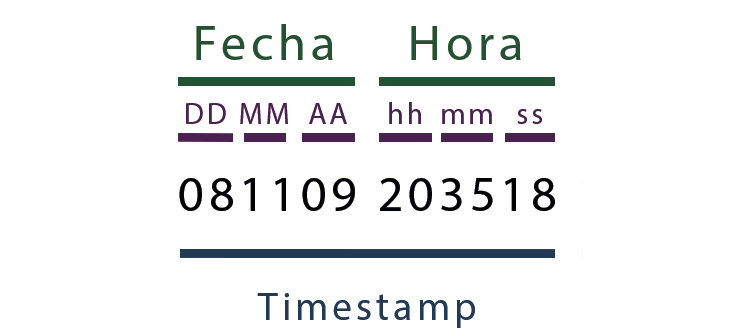
\includegraphics[width=0.6\linewidth]{imagenes/hdfs-log-structure-timestamp.png}
    \caption{Estructura del \textit{timestamp} de un \textit{log} de \gls{HDFS}}
    \label{fig:hdfs-log-structure-timestamp}
\end{figure}

Normalmente, todos los \textit{logs} de servicios software, dispositivos y otros sistemas operativos contienen los mismos campos. De hecho, para que un producto de este tipo pueda pasar una evaluación del tipo \gls{CC} (\textit{Common Criteria}) (reconocida a nivel mundial), es necesario que los registros de \textit{logs} cumplan con el \gls{SFR} \textit{FAU\_GEN.1}  \cite{commoncriteria}, el cual especifica el contenido mínimo que debe tener un evento registrado. \\

En conclusión, puede diferirse que los \textit{datasets} de eventos son de tipo no estructurado, por lo que pueden llevarse a cabo varios enfoques. Para este trabajo se hará un acercamiento mediante diferentes métodos de \textit{clustering} para poder detectar vectores de ataque y llevar a cabo agrupaciones de \textit{logs} para su posterior análisis. Previamente será necesario el preprocesado de los datos para unificar su formato, extrayendo más características importantes del campo \textit{message} junto con aquellas anteriormente mencionadas a través del uso de técnicas de \textit{parsing}.

\vspace{5mm}

% ********************************************************************

\section{Algoritmos de \textit{machine learning} escogidos}

Existen diversos métodos que abordan la clasificación y agrupamiento de \textit{logs} para poder detectar posibles patrones de ataque en sistemas Linux. Este Trabajo se centrará principalmente en el \textit{clustering} \cite{Aggarwal2013}. 

En primer lugar es necesario establecer una definición para esta técnica; en base a la proporcionada por \textit{Barreno Recio} et. al \cite{BarrenoRecio2023}.  \\

\begin{definition}
\shorthrule \vspace{0.1cm}
\\
El \textit{clustering} \label{clustering} se refiere al método de agrupación no supervisada de un conjunto de datos \(D = \{F_1, F_2, \ldots, F_n\}\) en \(k\) grupos \(C = \{C_1, C_2, \ldots, C_k\}\) utilizando una métrica de similitud diseñada para maximizar la homogeneidad entre los elementos de un mismo grupo y aumentar la heterogeneidad con respecto a los elementos de los otros grupos.
\\ \vspace{0.1cm}
\fullhrule
\end{definition}


De tal modo, la idea consiste en poder agrupar conjuntos de \textit{logs} que tengan características similares, de modo que entre dichas agrupaciones se encuentren vectores de ataque distintos como \gls{DoS} o fuerza bruta a servicios, como es el caso de la Figura \ref{fig:SSH-bruteforce-example}. Normalmente cuando se producen este tipo de ataques se genera una secuencia significativamente grande de eventos prácticamente equivalentes entre sí.

\begin{figure}[H]
    \centering
    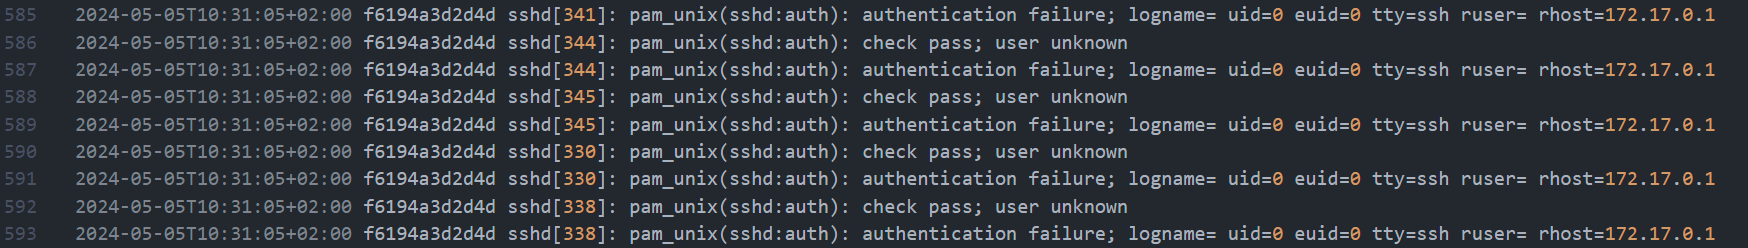
\includegraphics[width=1\linewidth]{imagenes/ssh-bruteforce-example.png}
    \caption{Ejemplo de secuencia de \textit{logs} generados por fuerza bruta a \gls{SSH}}
    \label{fig:SSH-bruteforce-example}
\end{figure}

Por tanto, basándonos en la definición anterior, el conjunto de datos D será un fichero que contenga una secuencia de eventos y estos serán agrupados en \textit{k} grupos de tipos de eventos distintos.

\newpage

\subsubsection*{Factores de un modelo de \textit{clustering}}

\setlist[itemize]{noitemsep, topsep=0pt}

\begin{table}[H]
\centering
\footnotesize
\renewcommand{\arraystretch}{0.9} 
\begin{tabularx}{\textwidth}{|>{\raggedright\arraybackslash}p{2.25cm}|>{\raggedright\arraybackslash}X|}
\hline
\rowcolor{graylight}\texttt{Factor} & \texttt{Descripción} \\
\hline
Representación de los datos & 
\begin{itemize}
    \item Adaptados: los datos son transformados para mejorar la estructura del modelo.
    \item No adaptados: los datos son utilizados en su forma original.
\end{itemize} \\
\hline
Medida de similitud & 
\begin{itemize}
    \item Tiempo: considerando las variaciones temporales.
    \item Cambio: observando las diferencias entre estados.
    \item Forma: evaluando la estructura de los datos.
\end{itemize} \\
\hline
Algoritmo de \textit{clustering} & 
\begin{itemize}
    \item Particional: K-Means, Fuzzy C-Means
    \item Jerárquico: \gls{AHC}, \gls{DHC}, \gls{HDBSCAN}, \gls{BIRCH}, \gls{FINCH}
    \item Densidad: \gls{DBSCAN}, \gls{OPTICS}, \gls{DENCLUE}, \gls{SNN}, \gls{DenMune}
    \item Cuadrícula: \gls{STING}, \gls{CLIQUE} 
\end{itemize} \\
\hline
Medidas de Evaluación &
\begin{itemize}
    \item Interna: \gls{KFCV}, \gls{LOOCV}
    \item Externa: uso de otros \textit{datasets} distintos al usado para el entrenamiento como \gls{HDFS}, \gls{BGL} o Linux\_2k.
\end{itemize} \\
\hline
\end{tabularx}
\caption{Factores de un modelo de \textit{clustering}}
\label{tab:clustering-factors}
\end{table}

\subsubsection*{Tipos de agrupamiento en técnicas de \textit{clustering}}

Además de los distintos factores indicados en la Tabla \ref{tab:clustering-factors}, se puede distinguir entre dos tipos de agrupamiento para el \textit{clustering}: el primero de ellos es el compacto, en el cual los elementos del grupo son muy parecidos y se representan a través de su punto central, mientras que el segundo es el agrupamiento encadenado \cite{https://doi.org/10.1002/widm.30}, en el cual un elemento de un grupo es más similar a otro de los elementos del grupo que los demás, produciéndose un efecto de cadena entre los elementos a través de una especie de ruta. Se puede ver en más detalle en la Figura \ref{fig:agrupamiento-clustering}.

\begin{figure}[H]
    \centering
    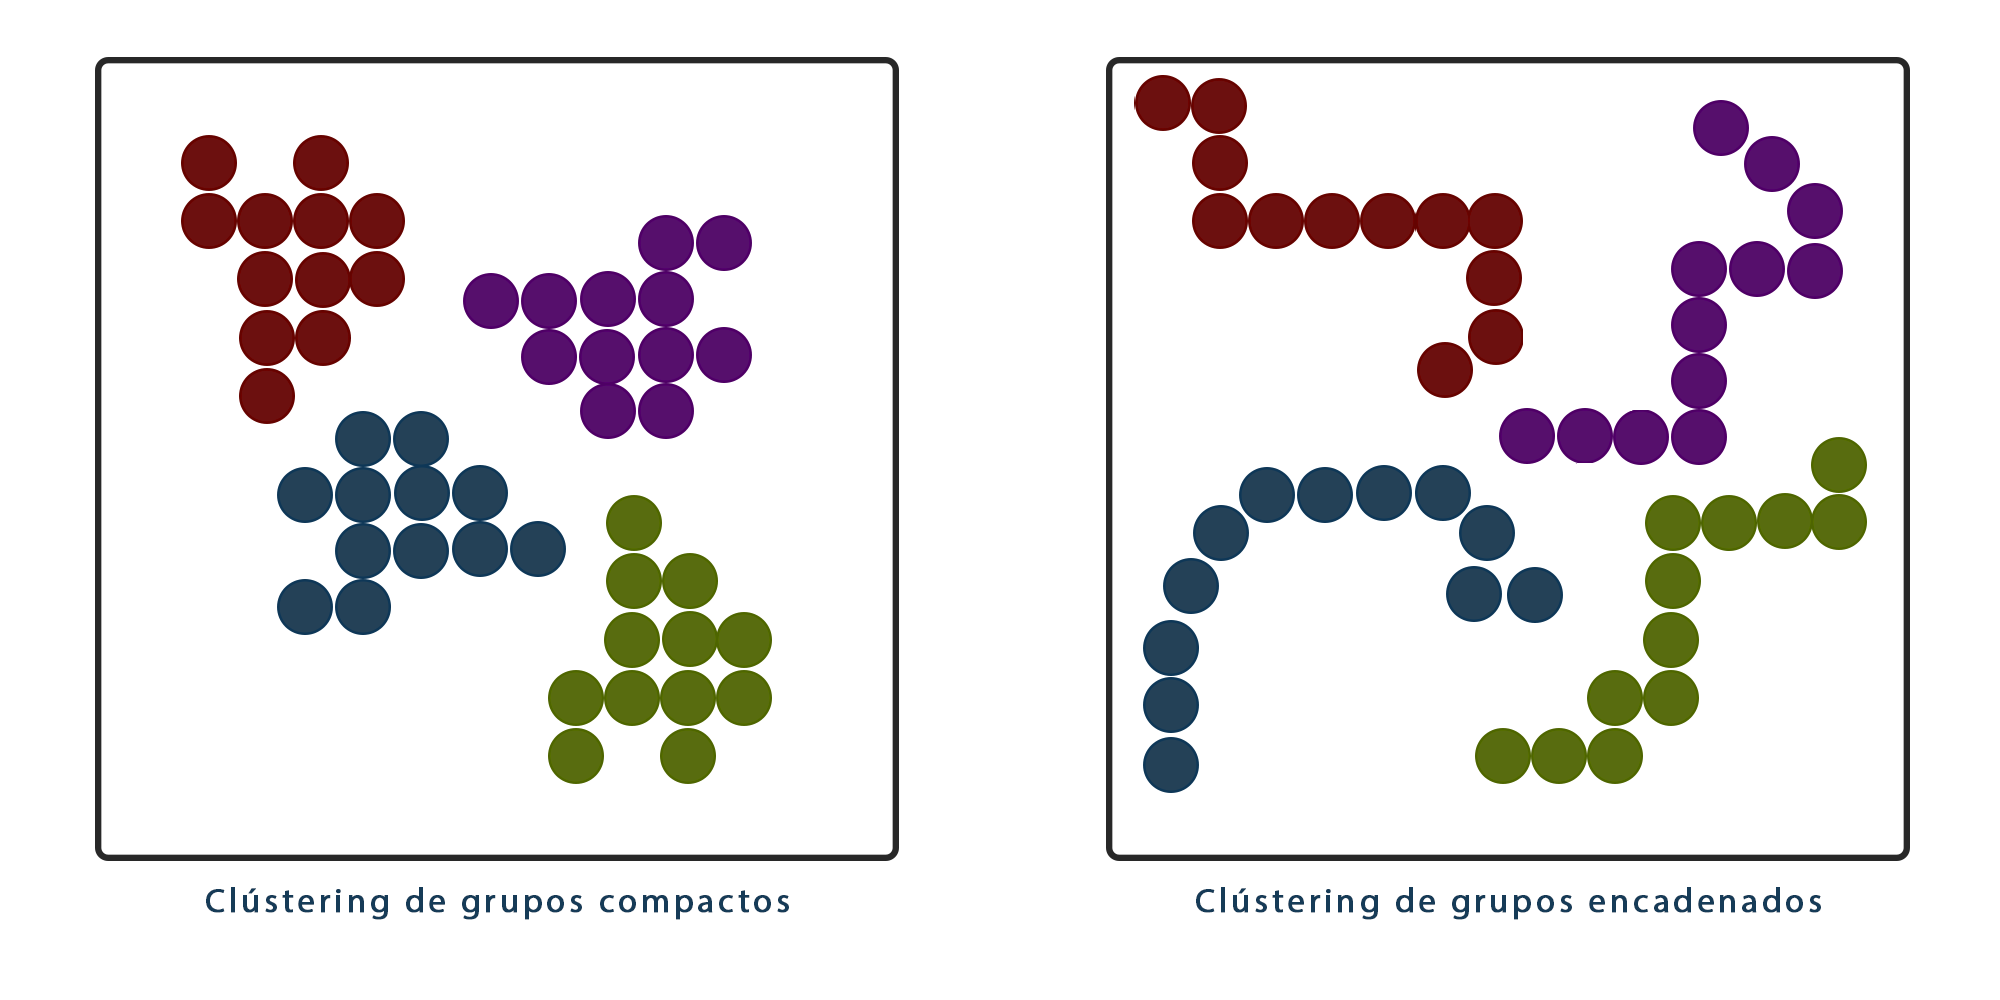
\includegraphics[width=0.75\linewidth]{imagenes/tipos-grupos-clustering.png}
    \caption{Tipos de agrupamiento en técnicas de \textit{clustering}} 
    \label{fig:agrupamiento-clustering}
\end{figure}

\newpage

\subsection{K-means}
\label{k-means}
Se trata de un algoritmo de \textit{clustering} basado en partición, es decir, este divide los datos en \textit{k} grupos de forma que cada grupo está compuesto por, al menos, un elemento. La forma de generar estos grupos consiste en tomar una serie de elementos que sean representativos, también conocidos como prototipos. 

La dificultad principalmente reside en escoger estos elementos representativos de manera que la partición sea lo más óptima posible. Para ello se lleva a cabo un proceso de iteración dividido en dos pasos:
\begin{itemize}
    \item Asignación: a partir de los prototipos iniciales se asignan los elementos al \textit{cluster} del prototipo que esté a menor distancia.
    \item Optimización: se vuelve a repetir el mismo proceso hasta que se cumpla una condición establecida, como un máximo de iteraciones o un error.
\end{itemize}

\vspace{-3mm}

\subsubsection*{Pseudocódigo del algoritmo K-means}

\vspace{-2mm}

\begin{myalgorithm}[H]
\footnotesize
\caption{K-means}
\textbf{Datos:} \textbf{D} Agrupación de datos a amontonar, \textbf{k} número de clúster\\
\textbf{Resultado:} Total de datos que forman \textit{D} agrupados en uno de los \textit{k} clúster
\begin{algorithmic}[1]
\State \textbf{Inicio;}
\State \textit{centroides} = lista de \textit{k} elementos aleatorios no repetidos de \textit{D};
\State \textit{clusters} = lista de \textit{k} clúster;
\Repeat
    \For{\textit{cada punto} $P$ \textbf{de} \textit{D}}
        \State \textit{centroideMasCercano} = centroides[0];
        \For{$c$ \textbf{en} \textit{centroides}}
            \If{$dist(P,c) < dist(P,centroideMasCercano)$}
                \State centroideMasCercano = $c$;
            \EndIf
        \EndFor
        \State Asignar $P$ al clúster al que pertenece centroideMasCercano;
    \EndFor
    \For{\textit{clust} \textbf{en} \textit{clusters}}
        \State Calcular Promedio del \textit{clust};
        \State Actualizar \textit{centroide};
    \EndFor
\Until{\textit{se cumplan un número de iteraciones, que todos los grupos cumplan una determinada tolerancia, que los grupos no cambien en esta iteración u otra condición de parada.}}
\end{algorithmic}
\end{myalgorithm}

\vspace{-0.3cm}

\subsubsection*{Parámetros del algoritmo K-means}

Este requiere de un único parámetro \textit{k}:

\begin{equation}
    Kmeans\ ( k )
\end{equation}

que es el número de \textit{clusters} en los que se quiere llevar a cabo el agrupamiento. \\

Su elección es crucial para obtener buenos resultados, es por ello que cuando no se conoce este valor es necesario aplicar una serie de heurísticas en base a la calidad de los grupos, como los gráficos de silueta \cite{10.1007/978-3-030-52348-0_2} o el método del codo (Figura \ref{fig:metodo-codo}), explicado por Syakur et. al \cite{Syakur_2018} en su artículo a través de los siguientes pasos:

\begin{enumerate}
    \item Determinar el número de \textit{clusters} \( K \) y el número máximo de iteraciones.
    \item Realizar el proceso de inicialización de los centroides de los clusters. La ecuación para calcular los centroides es:
    \begin{equation}
    C_i = \frac{1}{M} \sum_{j=1}^{M} x_j
    \end{equation}
    siendo \( M \) el número de datos asignados al cluster \( i \). 
    \item Asignar cada dato al \textit{cluster} más cercano utilizando la distancia euclidiana:
    \begin{equation}
    d = \sqrt{(x_1 - x_2)^2 + (y_1 - y_2)^2}
    \end{equation}
    \item Reasignar los datos a cada grupo basándose en la comparación de la distancia entre los datos y el centroide de cada grupo:
    \begin{equation}
    a_{ij} = \begin{cases} 
    1 & \text{si } d = \min \{D(x_i, c_i)\} \\
    0 & \text{en caso contrario}
    \end{cases}
    \end{equation}
    \item Recalcular la posición del centroide del cluster. La función objetivo \( J \) utilizada por este método se basa en la distancia y en el valor de la pertenencia de los datos al grupo:
    \begin{equation}
    J = \sum_{i=1}^{n} \sum_{l=1}^{k} a_{il} D(x_i, c_1)^2
    \end{equation}
    donde \( n \) es la cantidad de datos, \( k \) es el número de grupos, \( a_{il} \) es el valor de la pertenencia del punto de datos \( x_i \) al grupo \( c_1 \).
    \item Si hay un cambio en la posición del centroide del cluster o en el número de iteraciones, volver al paso 3. Si no, devolver el resultado del \textit{clustering}.
\end{enumerate}

\begin{figure}[H]
    \centering
    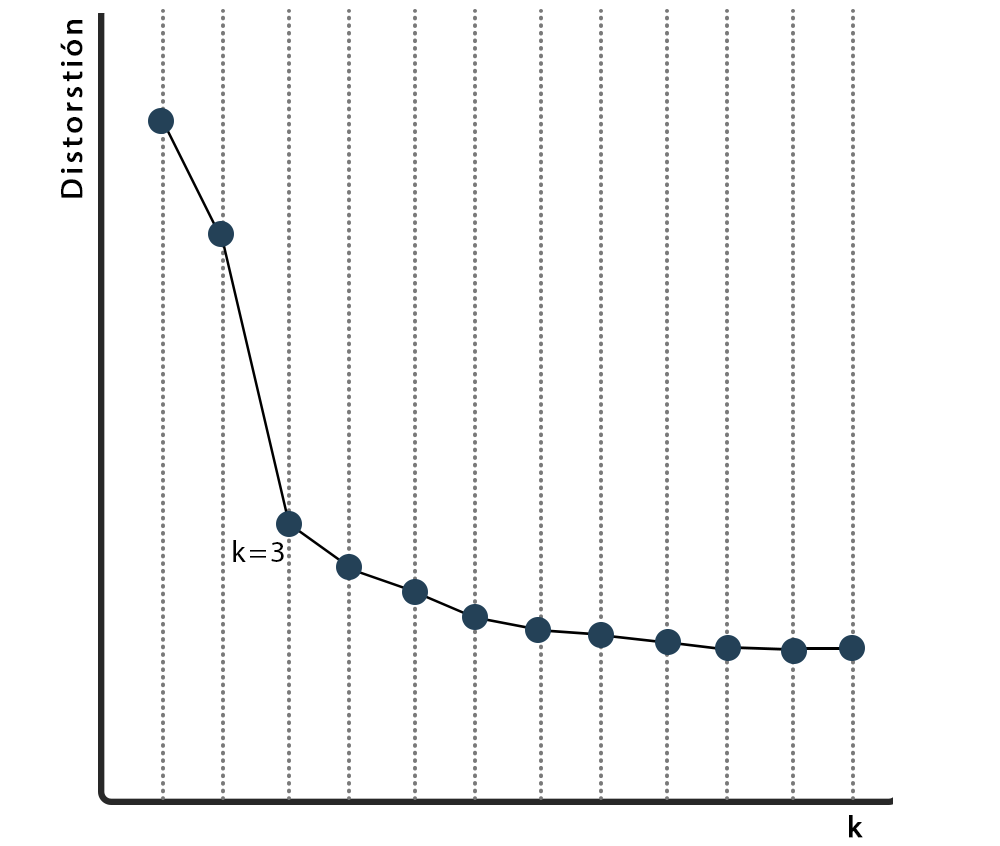
\includegraphics[width=0.75\linewidth]{imagenes/metodo-codo.png}
    \caption{Método del codo para la elección del parámetro \textit{k}}
    \label{fig:metodo-codo}
\end{figure}

\newpage

\subsubsection*{Orden de eficiencia de K-means}

Su orden de eficiencia es:

\vspace{-0.2cm}

\begin{equation}
    O(nkdi)
\end{equation}

donde \( n \) es el número de puntos de datos, \( k \) es el número de \textit{clusters}, \( d \) es la dimensión de los datos y \( i \) es el número de iteraciones hasta la convergencia. \\

\vspace{-3mm}

\subsubsection*{Librería sklearn para la implementación de K-means}

Puede aprovecharse la implementación del algoritmo K-means de la librería scikit-learn de Python \cite{datacamp_kmeans_2023}, la cual permite la normalización, ajuste y evaluación del modelo, así como la visualización de los resultados con un gran margen de personalización. \\

Consta de los siguientes parámetros de entrada y atributos de salida:

\begin{table}[H]
\centering
\footnotesize
\renewcommand{\arraystretch}{1.1}
\begin{tabularx}{\textwidth}{|p{3cm}|p{2.25cm}|X|}
\hline
\rowcolor{graylight}\texttt{Tipo} & \texttt{Nombre} & \texttt{Descripción} \\
\hline
\rowcolor{graylight}\multicolumn{3}{|c|}{\texttt{Parámetros de entrada}} \\
\hline
Parámetro & n\_clusters & Número de grupos en los que se dividen los datos. \\
\hline
Parámetro & init & Método que determina los centroides iniciales; permite las siguientes opciones:
\begin{itemize}
    \item \texttt{k-means++} \cite{arthur2007kmeans}: método por defecto.
    \item \texttt{random}: selecciona los centroides aleatoriamente.
    \item Matriz de centroides iniciales: se pueden pasar directamente.
\end{itemize} \\
\hline
Parámetro & n\_init & Número de repeticiones del algoritmo con diferentes centroides iniciales para obtener la mejor agrupación. \\
\hline
Parámetro & max\_iter & Número máximo de iteraciones para un conjunto dado de centroides iniciales. \\
\hline
\rowcolor{graylight}\multicolumn{3}{|c|}{\texttt{Atributos de salida}} \\
\hline
Atributo & cluster\_centers\_ & Array con los centroides de cada grupo, de dimensiones \( (k, m) \). \\
\hline
Atributo & labels\_ & Etiquetas de los elementos del conjunto agrupado, donde cada etiqueta i corresponde al centroide i en cluster\_centers\_. \\
\hline
Atributo & inertia\_ & Suma de las distancias al cuadrado de cada elemento a su centroide más cercano. \\
\hline
Atributo & n\_iter\_ & Número de iteraciones realizadas. \\
\hline
\end{tabularx}
\caption{Parámetros y atributos del algoritmo K-Means en sklearn}
\label{tab:kmeans}
\end{table}


\subsection{DBSCAN}
\label{dbscan}
Es el algoritmo de \textit{clustering} basado en densidad más utilizado en la actualidad \cite{10.1145/3068335} gracias a que no hace falta tener una gran base de conocimiento sobre los datos que se manejan y su uso es compatible con \textit{datasets} de gran tamaño.

Conceptualmente, \gls{DBSCAN} busca zonas que tengan una densidad alta y que estén alejadas de otras con una densidad más baja. 
Para ello se utilizan los términos \textit{neighbor}, que es un punto dentro del radio $\epsilon$ de otro punto, y \textit{neighborhood}, que es el conjunto de todos los puntos dentro del radio $\epsilon$ de un punto específico, incluyendo al punto mismo. \\

\begin{definition}
\shorthrule \vspace{0.1cm}
\\
El \textit{neighborhood} de un punto \( p \) conocido como \( N(p) \) puede definirse como:
\[
N(p) = \{ q \in D \mid \text{dist}(p, q) \leq \epsilon \}
\]
donde \( D \) es el conjunto de datos, \(\text{dist}(p, q)\) es la distancia entre los puntos \( p \) y \( q \), y \( \epsilon \) es el umbral de distancia.
\\ \vspace{0.1cm}
\fullhrule
\end{definition}

\subsubsection*{Pseudocódigo del algoritmo DBSCAN}

\begin{algorithm}[H]
\footnotesize
\caption{DBSCAN}
\textbf{Datos:} \textbf{D} conjunto de datos a agrupar, \textbf{eps} distancia máxima entre dos puntos vecinos, \textbf{minPts} mínimo número de puntos para formar un \textit{cluster}\\
\textbf{Resultado:} Datos agrupados en clusters
\begin{algorithmic}[1]
\State \textbf{Inicio;}
\State $C = 0$;
\For{\textit{cada punto} $P$ \textbf{de} \textit{D}}
    \If{$P$ \textit{no está en} \textit{visitados}}
        \State \textit{Marcar $P$ como visitado};
        \State $ptosVecinos = calcularRegion(P, eps)$;
        \If{$tamaño(ptosVecinos) < minPts$}
            \State \textit{marcar $P$ como ruido};
        \Else
            \State $C = próximo cluster$;
            \State $expandirCluster(P, ptosVecinos, C, eps, minPts)$;
        \EndIf
    \EndIf
\EndFor
\State \textbf{fin}
\end{algorithmic}
\end{algorithm}

Como se puede observar, se inicia desde un punto aleatorio y se verifica si en el radio \textit{eps} de ese punto existe un mínimo de puntos P. Si es así, se forma un \textit{cluster} y se vuelve a la primera etapa con uno de los puntos encontrados. Si no se alcanza el mínimo de puntos pero se ha llegado a través de un punto que sí cumplía esta condición, este formará parte del mismo \textit{cluster}. En caso de que no se pueda llegar al punto por medio de otros, no formará parte del \textit{cluster} y se clasificará como un nodo de tipo \textit{noise}.

\newpage

\subsubsection*{Parámetros del algoritmo \gls{DBSCAN}}

Los dos parámetros utilizados por este algoritmo son:

\begin{equation}
    DBSCAN ( eps, MinPts )
\end{equation}

donde

\begin{itemize}
    \item \textit{eps} es el radio máximo de un vecindario de un punto, es decir, la distancia máxima que se considera para definir los puntos vecinos.
    \item \textit{MinPts} es el número mínimo de puntos requeridos para formar un punto {\textcolor{darkgreen}{\textbf{core}}}. Un punto se considera un punto \textit{core} si hay al menos \textit{MinPts} puntos dentro de su vecindario (incluyendo el mismo punto).
\end{itemize}

\subsubsection*{Clasificación de puntos en un \textit{cluster} de \gls{DBSCAN}}

Los puntos se clasifican en tres tipos posibles, tal y como se describe en la Tabla \ref{tab:dbscan} y se ilustra en la Figura \ref{fig:puntos-dbscan}.

\begin{table}[H]
\centering
\footnotesize
\renewcommand{\arraystretch}{1.1}
\begin{tabularx}{\textwidth}{|p{3cm}|X|}
\hline
\rowcolor{graylight}\texttt{Tipo} & \texttt{Descripción} \\
\hline
\textbf{\textcolor{darkgreen}{\textbf{core}}} & Puntos interiores de un \textit{cluster} con un vecindario de radio $\epsilon$. \\
\hline
\textbf{\textcolor{blue}{\textbf{border}}} & Tienen menos de MinPts puntos en su vecindario de radio Epsilon, estando en el vecindario de algún punto \textcolor{darkgreen}{\textbf{core}}. \\
\hline
\textbf{\textcolor{red}{\textbf{noise}}} & Cualquier punto que no forma parte del \textcolor{darkgreen}{\textbf{core}} de un \textit{cluster} ni está en su frontera o \textcolor{blue}{\textbf{border}}. \\
\hline
\end{tabularx}
\caption{Clasificación de puntos en DBSCAN}
\label{tab:dbscan}
\end{table}

\vspace{-2mm}

\begin{figure}[H]
    \centering
    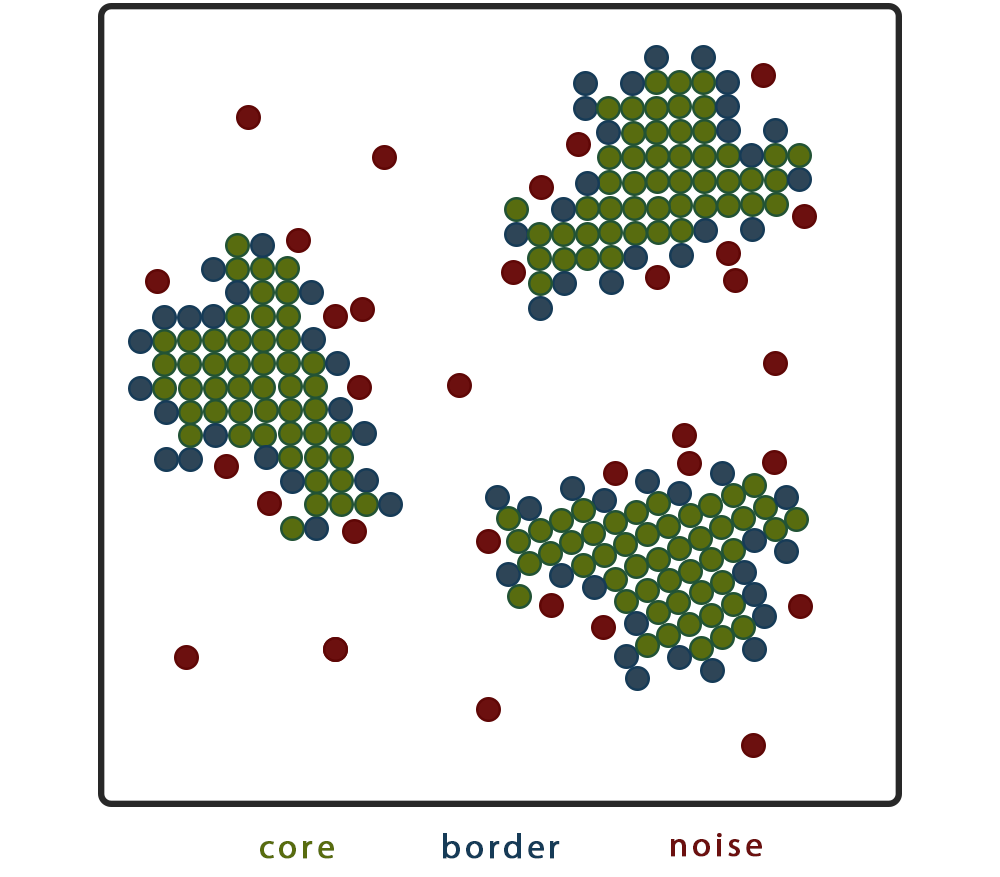
\includegraphics[width=0.725\linewidth]{imagenes/dbscan-points.png}
    \caption{Ejemplo de clasificación de puntos de algoritmo de \textit{clustering} \gls{DBSCAN}}
    \label{fig:puntos-dbscan}
\end{figure}

\subsubsection*{Orden de eficiencia de \gls{DBSCAN}}

Su orden de eficiencia es:

\vspace{-0.2cm}

\begin{equation}
    O(n \log n)
\end{equation}

donde \( n \) es el número de puntos de datos.

\subsection{Clustering Jerárquico} % clustering jerárquico. DHC También existe
\label{AHC}
También conocido como \textit{Agglomerative Hierarchical Clustering} \cite{Aggarwal2013}, este algoritmo jerárquico que agrupa datos de manera aglomerativa. Es decir, comienza tratando cada punto de datos como un clúster individual y, en cada paso, combina los dos clústeres más cercanos hasta que todos los puntos de datos pertenecen a un solo clúster.

El proceso del algoritmo se basa en la siguiente serie de pasos:

\begin{table}[H]
\footnotesize
\centering
\begin{tabular}{|l|p{12cm}|}
\hline
\rowcolor{graylight} \texttt{Paso} & \texttt{Descripción} \\
\hline
1 & Calcular la matriz de disimilitud entre todos los puntos de datos. \\
\hline
2 & Repetir los siguientes pasos hasta que quede un solo clúster: \\
\hline
3 & Fusionar los \textit{clusters} más cercanos \( C_a \) y \( C_b \). El nuevo \textit{cluster} tendrá una cardinalidad \( N_{a \cup b} = N_a + N_b \). \\
\hline
4 & Insertar una nueva fila y columna en la matriz de disimilitud que contenga las distancias entre el nuevo \textit{cluster} \( C_{a \cup b} \) y los \textit{clusters} restantes. \\
\hline
5 & Terminar cuando solo quede un \textit{cluster} máximo. \\
\hline
\end{tabular}
\caption{Pasos del algoritmo de Clustering Jerárquico Aglomerativo}
\end{table}


\vspace{-3mm}

\subsubsection*{Pseudocódigo del algoritmo \gls{AHC}}

\vspace{-3mm}

\begin{algorithm}[H]
\footnotesize
\caption{AHC}
\textbf{Datos:} \textbf{D} Agrupación de datos a amontonar\\
\textbf{Resultado:} Datos agrupados en un solo \textit{cluster} jerárquico
\begin{algorithmic}[1]
\State \textbf{Inicio;}
\State Calcular la matriz de disimilitud entre todos los puntos de datos;
\Repeat
    \State Fusionar los \textit{clusters} más cercanos $C_a \cup C_b$. Establecer la cardinalidad del nuevo \textit{cluster} como $N_{a \cup b} = N_a + N_b$;
    \State Insertar una nueva fila y columna que contenga las distancias entre el nuevo clúster $C_{a \cup b}$ y los \textit{clusters} restantes;
\Until{solo quede un \textit{cluster} máximo.}
\end{algorithmic}
\end{algorithm}

\vspace{-0.1cm}

\subsubsection*{Parámetros del algoritmo \gls{AHC}}

A diferencia de los anteriores, este algoritmo no requiere parámetros explícitos como K-means o \gls{DBSCAN}. En su lugar, la principal decisión que hay que tomar es la métrica de disimilitud \footnotemark utilizada para calcular las distancias entre \textit{clusters}, que puede ser:

\begin{itemize}
    \item Distancia simple (\textit{single linkage}): La distancia mínima entre puntos de diferentes \textit{clusters}. \\
    \item Distancia completa (\textit{complete linkage}): La distancia máxima entre puntos de diferentes \textit{clusters}.\\
    \item Distancia promedio (\textit{average linkage}): El promedio de todas las distancias entre puntos de diferentes \textit{clusters}.
\end{itemize}

\footnotetext{Es una medida que cuantifica cuán diferentes son dos elementos. En el contexto del \textit{clustering}, se utiliza para calcular la distancia entre puntos de datos o \textit{clusters}.}

\vspace{-3mm}

\subsubsection*{Orden de eficiencia de AHC}

El orden de eficiencia del algoritmo AHC es:

\vspace{-0.2cm}

\begin{equation}
    O(n^3)
\end{equation}

donde \( n \) es el número de puntos de datos. Este orden de eficiencia se debe al cálculo repetido de distancias entre todos los pares de clústeres a medida que se fusionan durante la construcción del árbol jerárquico. \\

Cuando se habla de \textit{clustering} jerárquico, debe definirse qué es un dendrograma. Se trata de una representación gráfica de los resultados del \textit{clustering} tal que en el eje vertical se muestra la distancia o disimilitud en la que se combinan los \textit{clusters}, mientras que en el eje horizontal se encuentran los puntos de datos, como se muestra en la Figura \ref{fig:dendrogram-example}. Esta visualización permite identificar la estructura del \textit{cluster} y decidir el número óptimo de \textit{clusters} al cortar el dendrograma a una altura específica.

\begin{figure}[H]
    \centering
    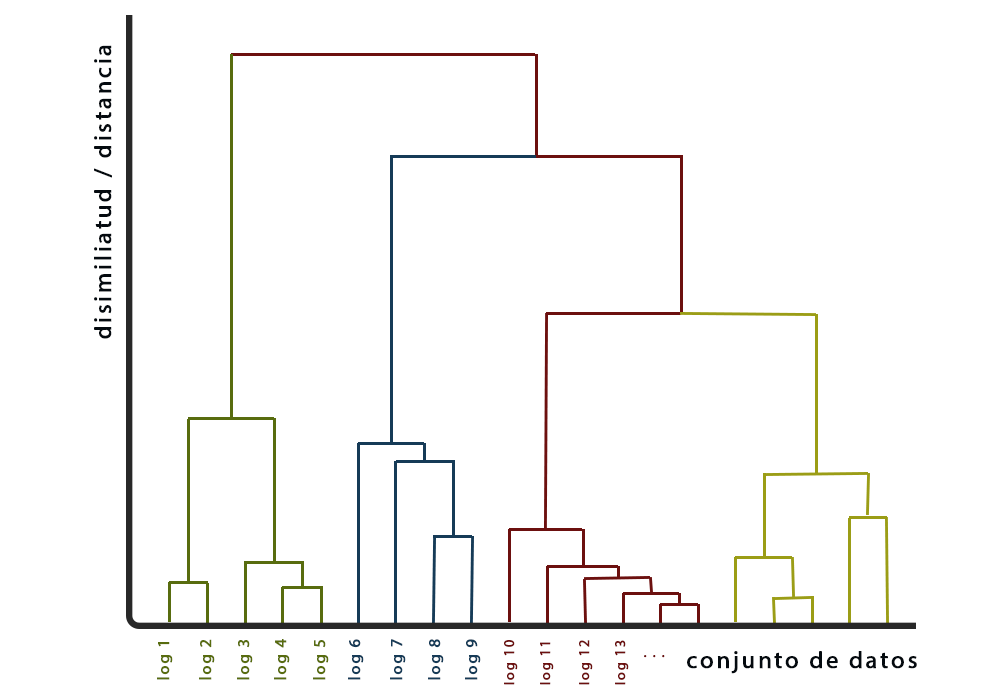
\includegraphics[width=0.8\linewidth]{imagenes/dendrograma.png}
    \caption{Ejemplo de un dendrograma para \gls{AHC}}
    \label{fig:dendrogram-example}
\end{figure}

\newpage

% ********************************************************************

\section{\textit{Set-up} experimental: tecnologías y herramientas}

\vspace{-1mm}

Para llevar a cabo la implementación del proyecto con la mayor precisión posible, se ha llevado a cabo un proceso minucioso de selección de las tecnologías y herramientas que se iban a utilizar.

\subsection{Herramientas para la simulación de ataques}

En primer lugar, ha sido necesario seleccionar uno de los múltiples \textit{frameworks} existentes basados en el marco adversario de  MITRE \gls{ATT&CK} para llevar a cabo la simulación de ataques a las máquinas y la posterior generación de grandes cantidades de \textit{logs} que pudiesen ser procesadas para generar un \textit{dataset}. Complementariamente, se han utilizado otras herramientas de explotación para enriquecer la cantidad de eventos generados a raíz de distintos ataques.

\vspace{-1mm}

\subsubsection*{Framework \gls{CALDERA}}

El \textit{framework} escogido ha sido \textbf{\gls{CALDERA}} \cite{caldera}, ya que permite emular la totalidad de técnicas y tácticas contempladas por el marco de MITRE, además de ofrecer una gran personalización. La versión utilizada ha sido la v5.0.0 "Magma" \cite{caldera_v500}, publicada el pasado 14 de febrero. A diferencia de las alternativas propuestas en la segunda sección del Estado del Arte (\ref{frameworks-mitre}), esta ha sido directamente desarrollada por MITRE, lo que la convierte en la solución opensource más estandarizada y utilizada en el entorno empresarial. 

Su funcionamiento está basado en la combinación de dos sistemas: \gls{ViRTS}, una infraestructura sofware usada para crear y emular adversarios de \textit{red-team}, y un modelo lógico denominado \gls{LAVA} que se encarga de determinar que acciones adversarias llevar a cabo. 

Por otro lado, la infraestructura de \gls{CALDERA}, instanciada por \gls{ViRTS}, se compone de dos elementos principales: el servidor maestro (ExtroViRTS) y los clientes de herramientas de acceso remoto (\gls{RAT}) en hosts ya infectados (IntroViRTS), como se observa en la Figura \ref{fig:caldera-infraestructure}. 

El proceso consta de los siguientes pasos \cite{gjerstad2022generating}:

\begin{enumerate}
    \item \textbf{Configuración inicial}: \gls{CALDERA} se configura de modo que un único host esté infectado con un \gls{RAT} de IntroViRTS, asegurando que la comunicación entre este \gls{RAT} y el servidor maestro ExtroViRTS sea fluida. 
    \item \textbf{Ampliación del control}: A partir de la infección inicial, \gls{CALDERA} utiliza el motor \gls{LAVA} para determinar las acciones a tomar. El servidor maestro ejecuta una instancia de LAVA para seleccionar una acción específica a ejecutar.
    \item \textbf{Ejecución de acciones}: El servidor maestro envía un comando a un \gls{RAT} específico en el campo, que ejecuta la acción seleccionada.
    \item \textbf{Retroalimentación y actualización}: El \gls{RAT} envía todos los detalles relevantes de la acción ejecutada de vuelta al servidor maestro.
    \item \textbf{Actualización de la base de conocimientos}: El servidor ExtroViRTS lleva a cabo la actualización de su base de conocimientos interna.
    \item \textbf{Selección de futuras acciones}: El servidor maestro continúa utilizando \gls{LAVA} para seleccionar futuras acciones que serán ejecutadas por los clientes IntroViRTS.
\end{enumerate}

\vspace{-3mm}

\begin{figure}[H]
    \centering
    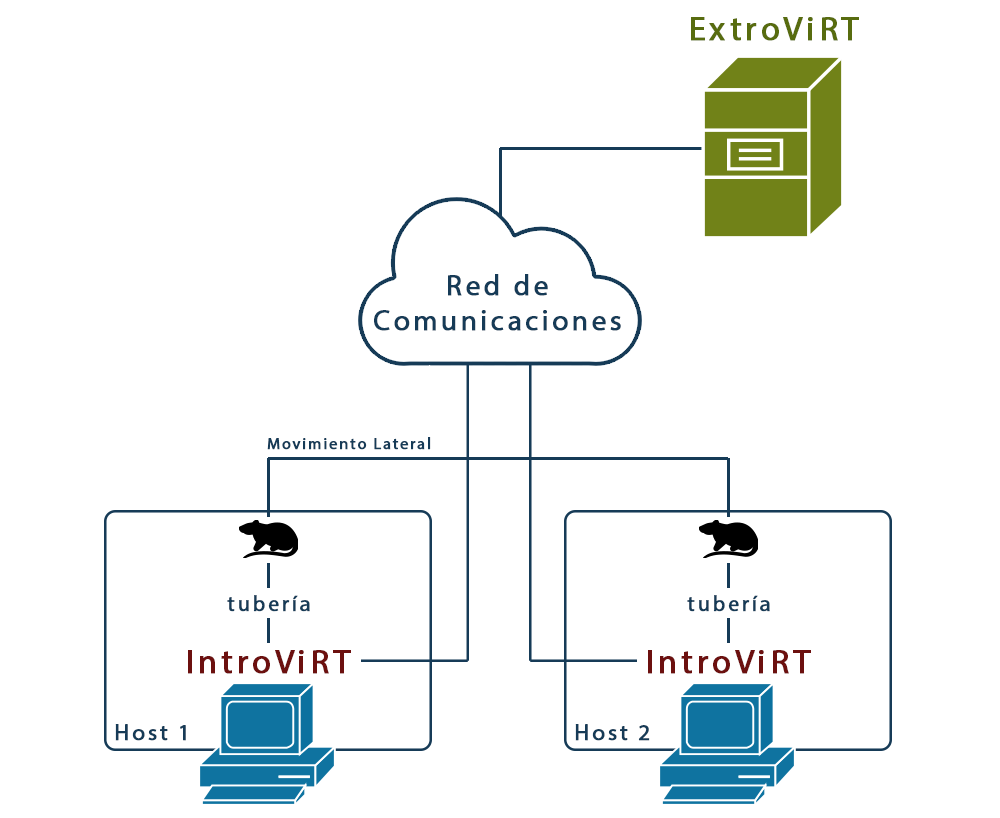
\includegraphics[width=0.75\linewidth]{imagenes/CALDERA-infraestructura.png}
    \caption{Infraestructura del framework \gls{CALDERA} \cite{gjerstad2022generating}}
    \label{fig:caldera-infraestructure}
\end{figure}

Este \textit{framework} emplea una terminología específica, cuyo entendimiento es vital para poder llevar a cabo un ataque. Como se muestra en la Tabla \ref{tab:caldera-terminologia}, distinguimos entre cuatro elementos principales:

\begin{table}[h]
\centering
\footnotesize
\begin{tabularx}{\linewidth}{|l|X|}
\hline
\rowcolor{graylight}\texttt{Término} & \texttt{Descripción} \\
\hline
Agentes & Aplicación software que se conecta de a CALDERA en intervalos regulares para obtener instrucciones. Cada agente se comunica con el servidor de CALDERA y se le asigna un ID único llamado \textit{paw}. Algunos ejemplos de agentes disponibles son Sandcat, Manx y Ragdoll. \\
\hline
Habilidades & Tácticas, técnicas y procedimientos específicos de ATT\&CK que se ejecutan en agentes activos. Cada habilidad incluye los comandos a ejecutar, las plataformas/ejecutores para el comando, cargas útiles y una referencia a los resultados de salida en el servidor de CALDERA. \\
\hline
Adversarios & Perfiles de amenazas predefinidos que consisten en un grupo de habilidades (\gls{TTP}s). Los perfiles pueden ayudar a determinar qué habilidades deberían ejecutarse al llevar a cabo una operación. \\
\hline
Operaciones & Ejecutan habilidades en grupos de agentes. \\
\hline
\end{tabularx}
\caption{Terminología utilizada por el \textit{framework} de \gls{CALDERA}}
\label{tab:caldera-terminologia}
\end{table}

En el próximo capítulo se documentará el proceso seguido para llevar a cabo la instalación y configuración del \textit{framework}.

\subsubsection*{Herramientas de ataque adicionales} \label{adicional-tools}

\gls{CALDERA}, según lo comentado anteriormente, basa su funcionamiento en la infección del host atacado mediante un \textit{payload} conocido como agente, es por ello que todos los ataques generados por este \textit{framework} están orientados a reconocimiento, movimiento lateral y otras operaciones de explotación y post-explotación. Por consiguiente, con la finalidad de aumentar la variedad de eventos recopilados en el \textit{dataset}, se hará uso de las siguientes herramientas de \textit{hacking} ético:

\begin{itemize}
    \item \texttt{Metasploit} \cite{Kennedy2011}: se trata del \textit{framework} más utilizado para ejercicios de \textit{pentesting}, es ampliamente conocido por facilitar la automatización de una amplia gama de ataques asociados a \gls{CVE}s. Cuenta con una gran base de datos, y su popularidad debe a la facilidad de uso para realizar ataques realistas y eficaces en entornos controlados.\\
    \item \texttt{Hydra} \cite{Beale2004}: es una herramienta de \textit{cracking} de contraseñas que destaca por su velocidad a través de opciones de ataques concurrentes mediante hebras, y su versatilidad, soportando múltiples protocolos de red. Es altamente efectiva en técnicas de fuerza bruta y ataques por diccionario.
\end{itemize}

\subsection{Virtualización de las máquinas víctima}

Para llevar a cabo la simulación de ataques, se investigó acerca de qué tecnología utilizar de cara al despliegue de \textit{hosts} que simularan una infraestructura operacional que hubiera sido vulnerada y tuviera un servidor central que almacenara internamente todos los eventos registrados. Las dos principales opciones eran las siguientes:

\begin{table}[h]
\centering
\footnotesize
\begin{tabularx}{\linewidth}{|l|X|}
\hline
\rowcolor{graylight}\texttt{Tecnología} & \texttt{Descripción} \\
\hline
Máquinas virtuales & Ofrecen un aislamiento completo del sistema operativo subyacente, lo que resulta en una mayor seguridad y estabilidad. Sin embargo, consumen más recursos y requieren más tiempo para configurarse y mantenerse en comparación con los contenedores. \\
\hline
Contenedores Docker & Permiten un despliegue rápido y eficiente, consumiendo menos recursos que las máquinas virtuales. Además, facilitan la portabilidad entre diferentes sistemas y plataformas. Sin embargo, ofrecen un aislamiento menor que las máquinas virtuales. \\
\hline
\end{tabularx}
\caption{Comparación de tecnologías de virtualización para la simulación de ataques}
\end{table}

Una tercera opción sería el uso de \gls{WSL} para realizar desde ahí la simulación de ataques, ya que desde el lanzamiento de la versión 2.0 se han implementado numerosas mejoras a nivel de aislamiento con respecto a Windows, y al mismo tiempo proporcionando cada vez una mayor funcionalidad, que previamente estaba muy limitada en la versión 1.0. 

Esto fue analizado el pasado 18 de mayo de 2024 en Hack-én por el investigador Sergio De Los Santos en su ponencia titulada \textit{\gls{WSL}: Windows Subsystem for Linux. Del odio al amor y del amor al odio}. En su libro recientemente publicado \cite{santos_wsl_2024} puede obtenerse mucha más información sobre el tema. 


\begin{figure}[H]
    \centering
    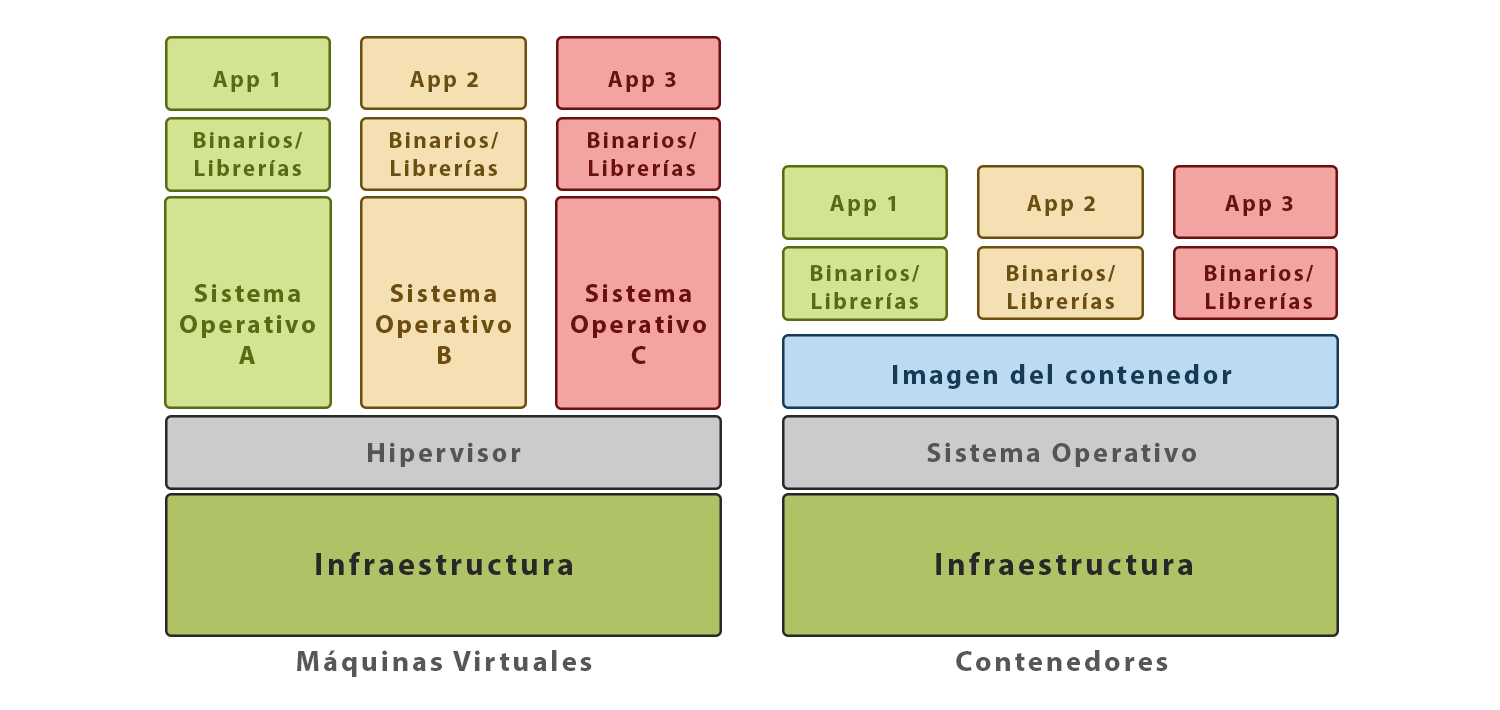
\includegraphics[width=1.1\linewidth]{imagenes/vms-vs-containers.png}
    \caption{Comparativa estructural de Máquinas Virtuales vs Contenedores}
    \label{fig:vm-vs-container}
\end{figure}

Finalmente, de las dos opciones ilustradas en la Figura \ref{fig:vm-vs-container} ha sido elegida la versión más ligera y simple: los contenedores \cite{vms_vs_containers}. Para el contexto de la simulación de ataques no suponía un problema que hubiese un menor aislamiento. Se llevaron a cabo pruebas de funcionalidad y rendimiento utilizando dos tipos de contenedores distintos.

El primero de ellos fue Alpine Linux \cite{alpine_linux}, que era la opción más ligera y rápida de generar a través de un Dockerfile, sin embargo tenía notables limitaciones y no representaba un entorno realista, ya que no se suele utilizar para servidores. La segunda opción fue un contenedor de Ubuntu Server \cite{ubuntu_server}, que ha resultado ser la elección definitiva, ya que sigue siendo una alternativa ligera pero con una utilidad suficiente como para llevar a cabo la simulación de ataques, y además es una distribución muy utilizada en cuanto a ingeniería de servidores respecta.

En el próximo capítulo se detallará cómo se ha llevado a cabo la implementación de los ficheros Dockerfile para levantar dichos contenedores.

\subsection{Librerías de Python utilizadas}

Python es actualmente el principal lenguaje de programación de alto nivel utilizado para cualquier actividad relacionada con análisis de datos, \gls{ML} o \gls{DL} \cite{subasi2020practical}. Es por ello que existen multitud de librerías que ofrecen una capa de abstracción para hacer uso de funcionalidades que se basan en el álgebra lineal y su implementación desde cero tendría un nivel de complejidad exponencial.

\vspace{-2mm}

\newpage

\subsubsection*{Librerías para el preprocesado de \textit{datasets}}

En primer lugar, para llevar acabo el preprocesado de \textit{datasets}, se han utilizado las siguientes librerías:

\begin{itemize}
\item \texttt{\gls{Pandas}}: Esta librería es una de las más conocidas en el análisis de datos. Proporciona estructuras de datos flexibles y potentes, conocidas como DataFrames, que facilitan la limpieza, transformación y análisis de grandes volúmenes de datos. Pandas permite cargar datos desde diversos formatos (CSV, Excel, SQL, etc.) y realizar operaciones complejas de agrupación, filtrado y agregación de manera eficiente. \\
\item \texttt{\gls{re}}: El módulo \textit{re} de Python proporciona soporte para expresiones regulares. Este permite buscar, sustituir y dividir cadenas de texto basándose en patrones específicos, lo cual resulta especialmente útil para el procesamiento de campos de \textit{logs}. \\
\item \texttt{\gls{CSV}}: La librería \textit{csv} se utiliza para leer y escribir archivos en formato \gls{CSV} (Comma-Separated Values). Este formato es el más utilizado para el análisis de datos y es compatible con muchas herramientas de análisis como las utilizadas en este proyecto para la implementación del \textit{clustering}. \\
\item \texttt{io}: El módulo \textit{io} de Python sirve para trabajar con flujos de datos en memoria, permitiendo la lectura y escritura de datos en diversos formatos sin necesidad de interactuar directamente con el sistema de archivos. Esto es útil para la manipulación temporal de datos durante el preprocesado.
\end{itemize}

El uso de estas librerías ha sido más que suficiente para realizar el preprocesado de los \textit{datasets} en un formato inicial de \texttt{.log}, ya que han permitido limpiar y posteriormente transformar los datos de manera eficiente de cara a su posterior análisis.

\subsubsection*{Librerías para la implementación del \textit{clustering}}

En segundo lugar, para la implementación de técnicas de \textit{clustering} en Python, se ha hecho uso de varias librerías que ofrecen un uso a alto nivel de algoritmos utilizados para la agrupación de datos como los estudiados anteriormente \ref{clustering}. Estas son:

\begin{itemize}
\item \texttt{Scikit-learn} (sklearn)\label{scikit}: Esta librería es una de las más populares para el aprendizaje automático en Python. Incluye una amplia gama de algoritmos de \textit{clustering}, como K-means, \glspl{DBSCAN} y \textit{clustering} jerárquico. Scikit-learn proporciona una interfaz sencilla y consistente para entrenar, evaluar y ajustar modelos, lo que facilita enormemente la integración de técnicas de \textit{clustering} en \textit{pipelines} de procesamiento de datos. \\
\item \texttt{NumPy}: Ofrece una poderosa estructura de datos en forma de arrays y matrices multidimensionales, y además permite realizar cálculos numéricos de forma eficiente sobre grandes volúmenes de datos, facilitando así la implementación de algoritmos de \textit{clustering} y otras técnicas de procesamiento de datos. \\
\item \texttt{Matplotlib}: Aunque no es una librería de \textit{clustering}, \textit{matplotlib} es fundamental para la visualización de los resultados del \textit{clustering}. Permite crear gráficos Y por tanto visualizar los resultados de los algoritmos de agrupación de cara a su análisis. \\
\item \texttt{Scipy}: Esta librería complementa a \textit{scikit-learn} proporcionando funciones adicionales para el análisis y manipulación de datos. Incluye herramientas para la implementación de \textit{clustering} jerárquico y otras técnicas similares. \\
\item \texttt{\gls{UMAP}-learn}: Tal y como indica su nombre, implementa la técnica de reducción de dimensionalidad que también se puede utilizar para el \textit{clustering}. \texttt{\gls{UMAP}} es especialmente útil para visualizar datos de alta dimensionalidad y descubrir estructuras subyacentes en los datos. Esto ha optimizado considerablemente la implementación del proyecto.  \\
\item \texttt{Tabulate}: Facilita la creación de tablas con diferentes estilos de formato de manera muy sencilla y rápida a partir de listas de datos o estructuras similares. Esta soporta texto simple, \gls{HTML}, LaTeX, y Markdown, lo cual resulta especialmente de cara al análisis de resultados.
\end{itemize}

El uso combinado de estas librerías ha permitido implementar de manera eficiente y robusta diversas técnicas de \textit{clustering}, que luego han sido utilizadas en los \textit{datasets} de \textit{logs} generados, para llevar a cabo el estudio de vectores de ataque.

\vspace{4mm}
\noindent\rule[-1ex]{\textwidth}{0.5pt}\\
\vspace{4mm}

En la Figura \ref{fig:diagrama-estructural} se muestra el diagrama estructural utilizado para llevar a cabo este Trabajo.

\newpage

\begin{landscape}   
    \noindent\hspace*{-2.7cm}
    \begin{minipage}{\linewidth}
        \begin{figure}[H]
            \centering
            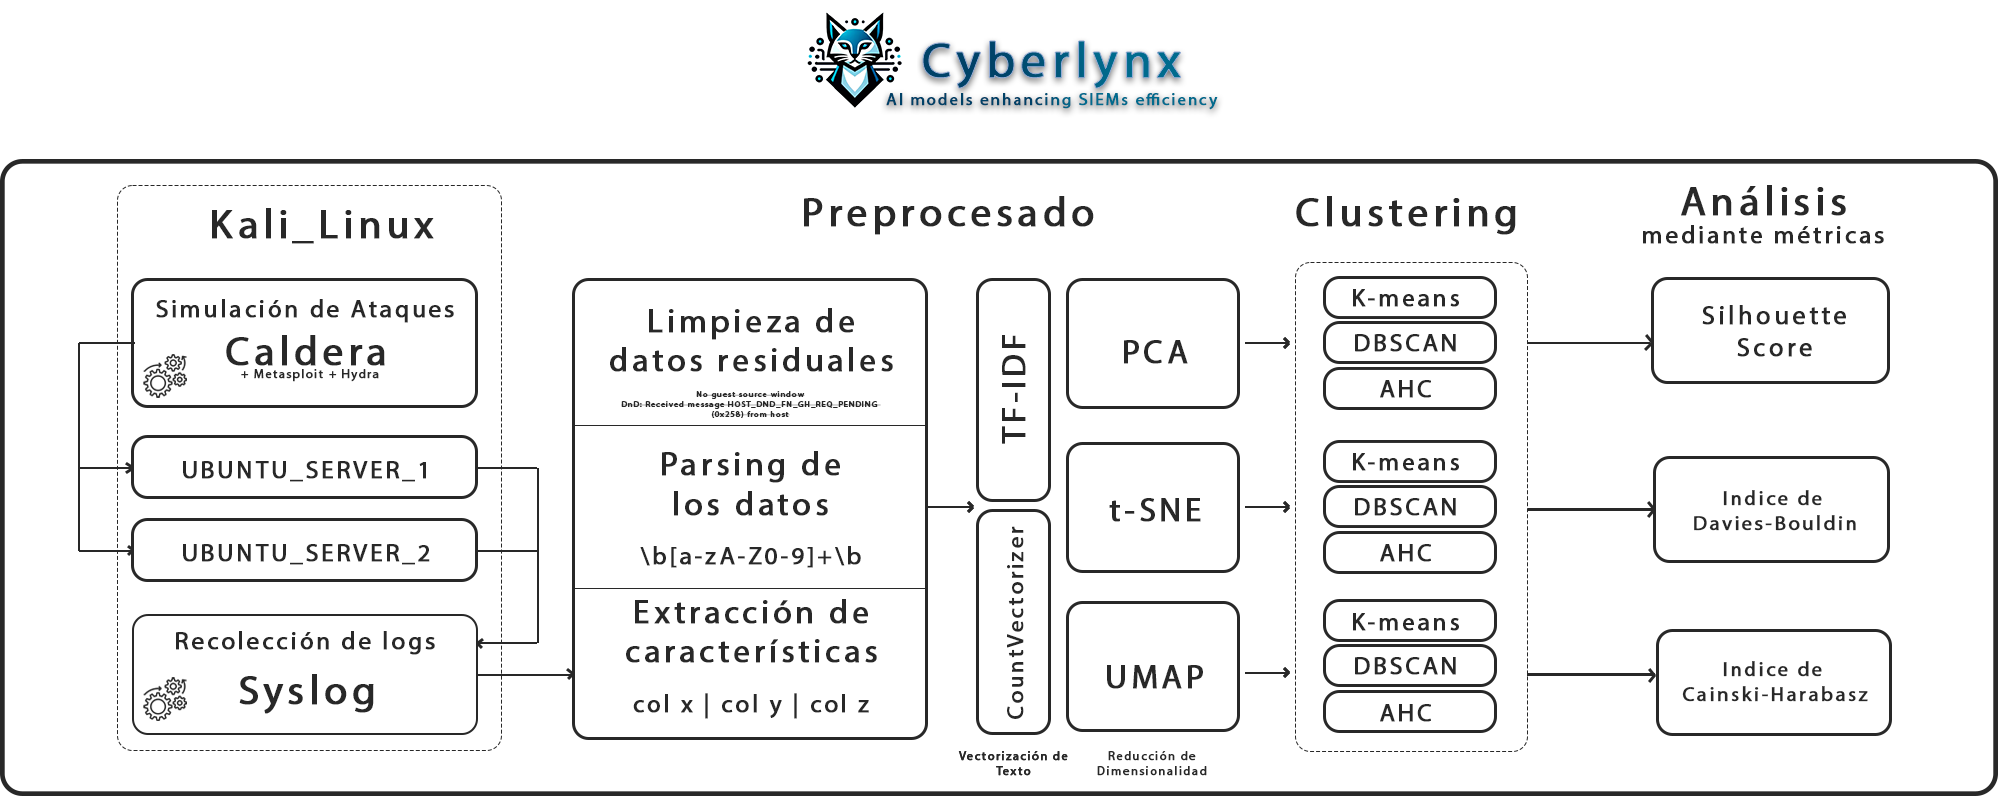
\includegraphics[width=1.3\linewidth, keepaspectratio]{imagenes/scheme-v4.png}
            \caption{Diagrama estructural del Trabajo de Fin de Grado}
            \label{fig:diagrama-estructural}
        \end{figure}
    \end{minipage}
\end{landscape}

\newpage